\documentclass[10pt,pdf,hyperref={unicode}]{beamer}
\usepackage[utf8]{inputenc}
\usepackage[russian]{babel}

\usetheme{Berlin}


\title{Алгоритм Шеннона --- Фано}
\author{Сирота Александр\newline\scriptsize github.com/nukefluke}
\institute{\normalsize{ГУАП} \\ \scriptsize{5 факультет \\ Группа 5511}}
\date[3pt]{\scriptsize{Санкт-Петербург, 2016}}
\thispagestyle{empty}

\setbeamertemplate{frametitle}[default][center]
\setbeamertemplate{footline}[frame number]

\begin{document}

\maketitle

\begin{frame}[t]\frametitle{Содержание}
	\tableofcontents
\end{frame}

\section{Основные сведения}
\subsection{}

	\begin{frame}[t]\frametitle{Создатели и идея алгоритма}
		\textbf{Алгоритм Шеннона --- Фано} --- один из первых алгоритмов 
		сжатия, который сформулировали американские учёные Клод Шеннон и Роберт 
		Фано.\\
		\vspace{1em}
		Главная идея алгоритма --- заменить часто встречающиеся символы более короткими кодами, а редко встречающиеся символы более длинными кодами.\\
		\vspace{1em}
		Алгоритм:
		\begin{itemize}
			\item Относится к вероятностным методам сжатия
			\item Использует коды переменной длины
			\item Использует префиксный код
		\end{itemize}
	\end{frame}

	\begin{frame}\frametitle{Методы алгоритма}
		\textbf{Вероятностные методы сжатия} опираются на частоту встречаемости символа в тексте.\\
		\vspace{1em}
		При использовании \textbf{кодов переменной длины} символы кодируются 
		набором бит различной длины.
		Часто встречающийся символ кодируется кодом меньшей длины, 
		редко встречающийся --- кодом большей длины.\\
		\vspace{1em}
		\textbf{Префиксный код} --- код, в котором 
		никакое кодовое слово не является префиксом какого-то другого кодового слова.
	\end{frame}

	\begin{frame}[t]\frametitle{Префиксное кодирование}
		Префиксное кодирование необходимо для однозначного\\
		разбиения закодированной последовательности на слова.

		Например, код, состоящий из слов 

		$$
			0 \quad 10 \quad 11 
		$$
		является префиксным, и сообщение 
		$$01001101110 $$
		можно разбить на слова единственным образом:
		$$
			0\quad10\quad0\quad11\quad0\quad11\quad10
		$$
	\end{frame}

	\begin{frame}[t]\frametitle{Префиксное кодирование}
		Код, состоящий из слов 
		$$
			0\quad10\quad11\quad100
		$$

		префиксным не является (cлово $10$ является префиксом слова $100$), и то же сообщение можно трактовать уже несколькими способами.
		$$
			0\quad10\quad0\quad11\quad0\quad11\quad10
		$$$$
			0\quad100\quad11\quad0\quad11\quad10
		$$
	\end{frame}

\section{Построение кодов}
\subsection{}

	\begin{frame}[t]
		\frametitle{Алгоритм построения кодов}
		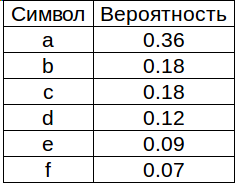
\includegraphics[height=10em]{alg0.png}
		\vspace{1em}
		\newline
		Для начала мы должны определиться, какие символы встречаются чаще, а какие реже.
		Необходимо проанализировать кодируемое сообщение и создать таблицу вероятностей.\\

	\end{frame}

	\begin{frame}[t]
		\frametitle{Алгоритм построения кодов}
		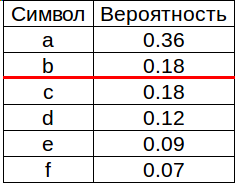
\includegraphics[height=10em]{alg1.png}
		\vspace{1em}
		\newline
		Далее, таблица символов делится на две группы таким образом,
		чтобы каждая из групп имела приблизительно одинаковую частоту
		по сумме символов.\\
		Это отличие алгоритма Фано от других подобных алгоритмов.\\
		
	\end{frame}

	\begin{frame}[t]
		\frametitle{Алгоритм построения кодов}
		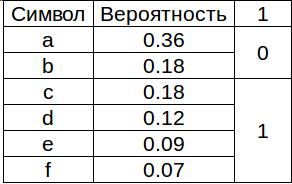
\includegraphics[height=10em]{alg2.png}
		\vspace{1em}
		\newline
		Первой группе устанавливается начало кода в '0', второй в '1'.\\
		
	\end{frame}

	\begin{frame}[t]
		\frametitle{Алгоритм построения кодов}
		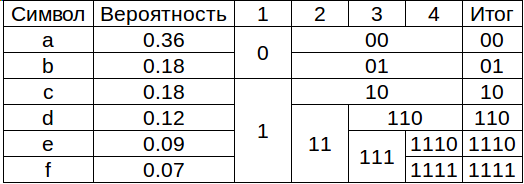
\includegraphics[height=10em]{alg3.png}
		\vspace{1em}
		\newline
		Процедура рекурсивно повторяется, пока в группе не останется только один символ.\\
		
	\end{frame}

	\begin{frame}
		\frametitle{Итого}
		Алгоритм Фано:
		\begin{enumerate}
			\item Выписать символы по убыванию вероятностей.
			\item Разделить список на две части с равными долями вероятности.
			\item Для первой части добавить к коду <<0>>, для второй --- <<1>>.
			\item Повторить шаги (1--3) для каждой части.
		\end{enumerate}
	\end{frame}

\section{Бинарное дерево}
\subsection{}

	\begin{frame}
		\frametitle{Бинарное дерево}
			Для построения кодов удобно использовать бинарное дерево, так как 
			после построения коды элементов-листьев получаются префиксными.
		\begin{itemize}
			\item Корень дерева --- весь алфавит
			\item После разбиения группы на две подгруппы, каждая подгруппа образует узел
			\item Ветви до этих узлов обозначаются '0' и '1'
			\item Если в группе один элемент, то группа образует лист дерева
			\item Код элемента - это последовательность цифр на ветвях, которые ведут от корня к этому элементу
		\end{itemize}

	\end{frame}

	\begin{frame}
		\frametitle{Пример кодового дерева}
			
		\begin{figure}
			\begin{minipage}{0.25\textwidth}
			\raggedright{\scriptsize{Исходные символы:}}
			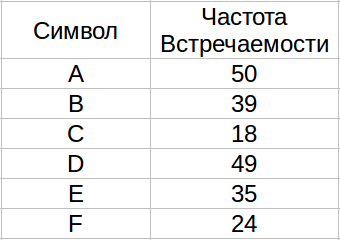
\includegraphics[width=\textwidth]{tree_sym.png}
			\end{minipage}
			\begin{minipage}{0.74\textwidth}
			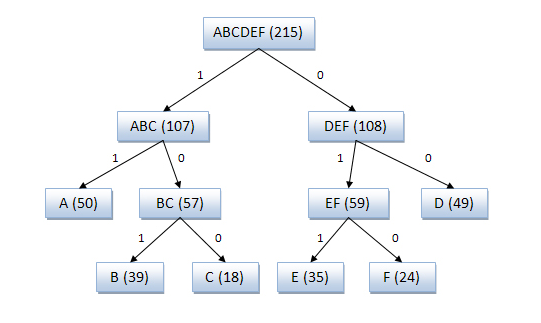
\includegraphics[width=\textwidth, trim= 20 20 50 15, clip=true]{tree.png}
			\end{minipage}
		\raggedright{Полученные коды:}
		
		\vspace{1em}
		\begin{minipage}[b]{\textwidth}
			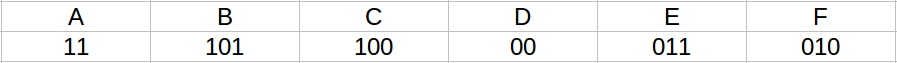
\includegraphics[width=\textwidth]{tree_code.png}
		\end{minipage}
		\end{figure}
	\end{frame}

\section{Реализация}
\subsection{}

	\begin{frame}[t]\frametitle{Проблемы реализации}
			\begin{itemize}
				\item Иногда коды строятся неоптимально.\\
					Например, коды для последовательности\\
					<<aaaaaaaaaaaaaabbbbbbbcccccdddddeeee>>:\\
					\vspace{1em}
					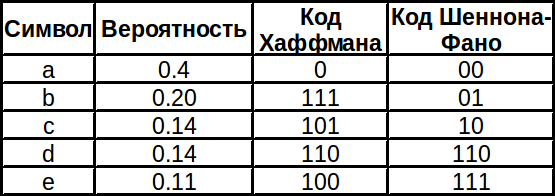
\includegraphics[height=6em]{fano-haff.png}\\
					\vspace{1em}
					Метод Хаффмана сжимает её до 77 бит, а Шеннона-Фано до 79 бит.
				\item Необходимо дописывать шапку в файл.
					Шапка содержит информацию о том, какие символы кодируются той или иной последовательностью.
			\end{itemize}
	\end{frame}

	\begin{frame}
		\frametitle{Интерфейс}
		\begin{block}{Запуск программы}
			\$ ./fano <mode> <input> [ -o <output> ]
		\end{block}
		\begin{exampleblock}{<mode>}
			\textbf{'-e'} --- кодирование. Расширение входного файла --- любое.\\
			\textbf{'-d'} --- раскодирование. Расширение входного файла \textbf{.fano}
		\end{exampleblock}
		\begin{exampleblock}{<input>}
			Входной файл.
		\end{exampleblock}
		\begin{exampleblock}{<output>}
			Выходной файл.
		\end{exampleblock}
	\end{frame}

	\begin{frame}
		\frametitle{Пример сгенерированного словаря}
		Для фразы:

		\vspace{1em}
		\scriptsize{\textit{<<Lorem ipsum dolor sit amet, consectetur adipisicing elit. 
		Odit sint cupiditate magni, illo officia facere magnam, ad pariatur ipsum explicabo 
		sit nostrum aliquid nisi necessitatibus natus temporibus. Ut, optio, odit.>>}}

		\vspace{1em}
		\centerline{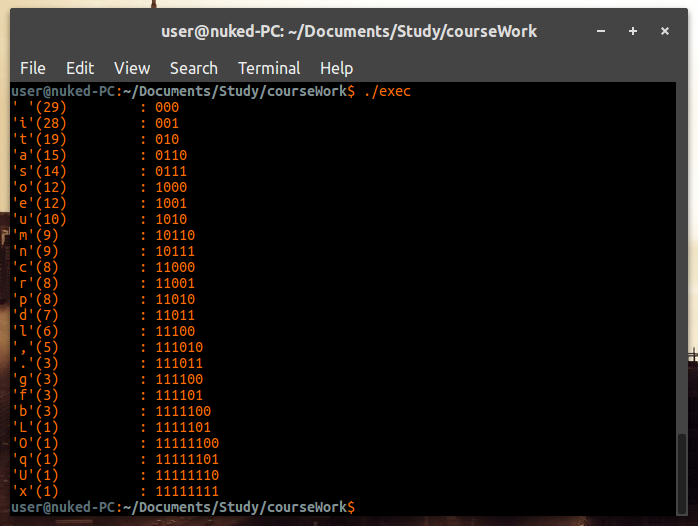
\includegraphics[height=20em]{gen.png}}
	\end{frame}

	\begin{frame}
		\frametitle{Оценка сложности}
		Кодирование файла:\\ 
		\begin{itemize}
			\item Подсчёт символов: $O(n)$
			\item Построение дерева: $O(c)$
			\item Создание шапки для закодированного файла: $O(c)$
			\item Запись закодированных данных в файл: $O(n)$
		\end{itemize}
		Раскодирование файла:\\ 
		\begin{itemize}
			\item Чтение шапки: $O(c)$
			\item Создание таблицы кодировки: $O(c)$
			\item Раскодирование: $O(n)$
			\item Запись раскодированных данных в файл: $O(n)$
		\end{itemize}
		
		Итоговая сложность --- линейная $O(n)$
	\end{frame}

	\begin{frame}
		\frametitle{Исходный код}
		\begin{block}{Репозиторий на github}
			https://github.com/nukefluke/fano-algorithm
		\end{block}
	\end{frame}

\section{Эффективность}
\subsection{}

\begin{frame}\frametitle{Текстовый файл}
	При сжатии текстового файла, содержащего один миллион слов~(7,6~Мб), 
	получился файл размером 4~Мб. Эффективность сжатия - 47\%.\newline

	\centering
	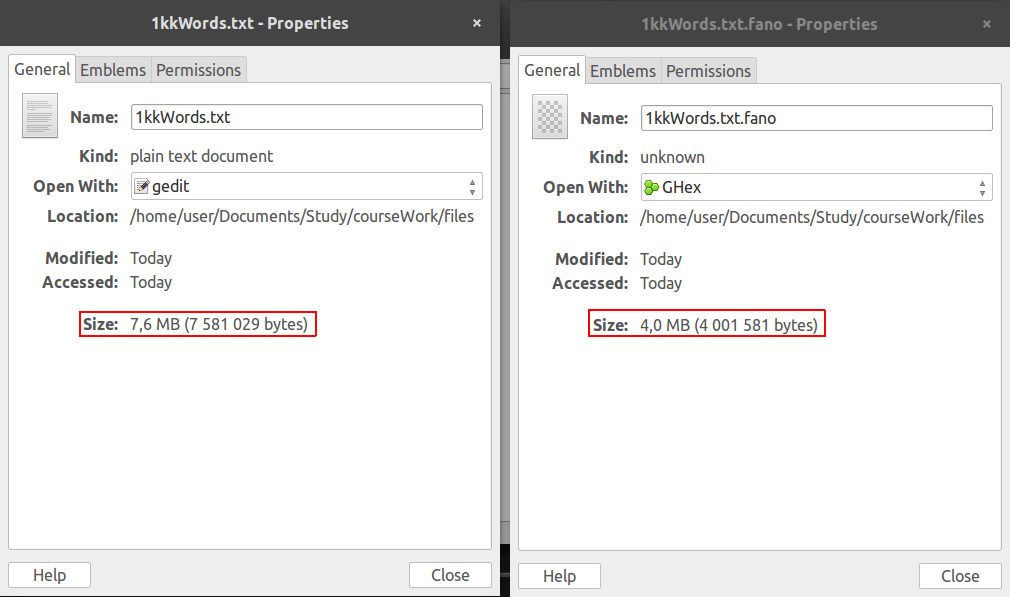
\includegraphics[width=0.8\textwidth]{compare.png}
\end{frame}

\begin{frame}\frametitle{Программа}
		При сжатии программой самой себя~(158.5~Кб), 
		получился файл размером 117.8~Кб. Эффективность сжатия - 25\%.\newline

		\centering
		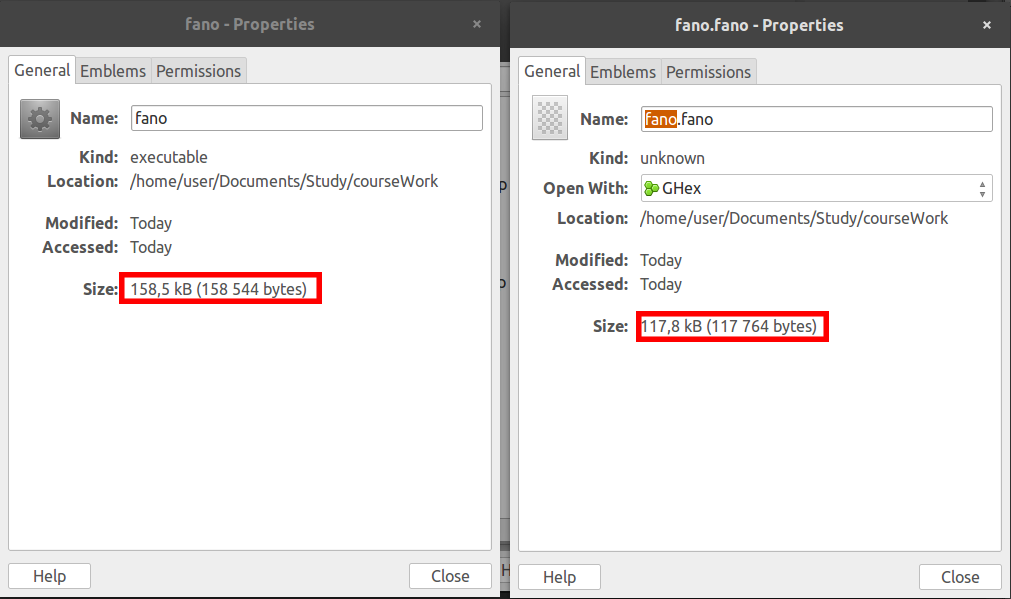
\includegraphics[width=0.8\textwidth]{compare1.png}
\end{frame}

\begin{frame}\frametitle{Пиксельный рисунок}
		При сжатии рисунка~(71,7~Кб), 
		получился файл размером 72,1~Кб. Здесь сжатие показало 
		отрицательную эффективность.\newline

		\centering
		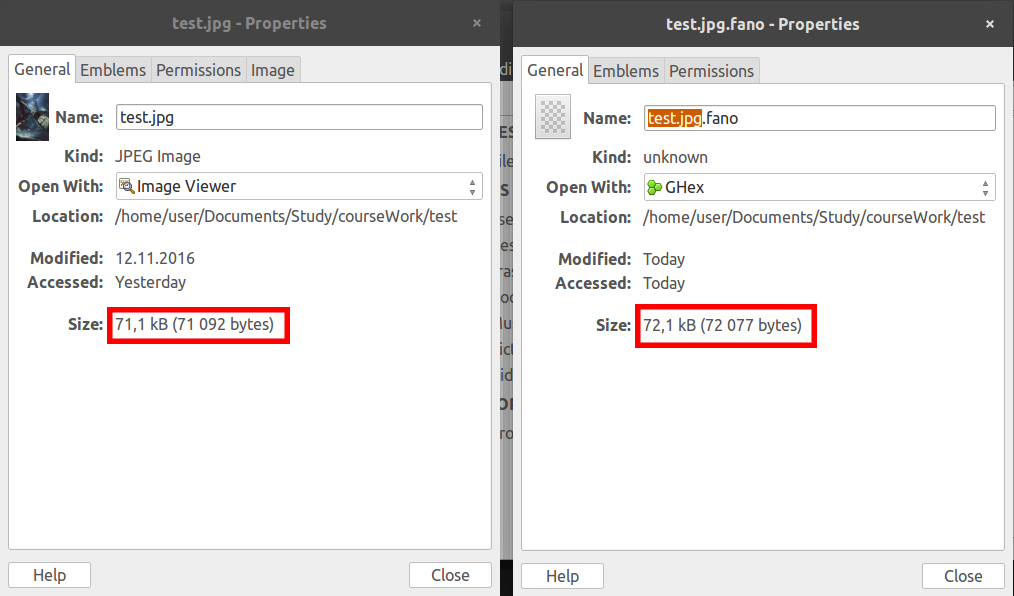
\includegraphics[width=0.8\textwidth]{compare2.png}
\end{frame}

\section{Итоги}
\subsection{}

\begin{frame}[t]\frametitle{Итоги}
	\begin{itemize}
		\item Алгоритм Шеннона --- Фано вероятностный, использует коды переменной длины
		\item Для построения кодов используется бинарное дерево
		\item Программа работает быстро --- линейная сложность
		\item Эффективность сжатия может быть отрицательной
	\end{itemize}

\end{frame}

\section{}

\begin{frame}
	\thispagestyle{empty}
	\centerline{Спасибо за внимание!}
\end{frame}

\end{document}